\ifx\allfiles\undefined
\documentclass[UTF8]{ctexart}
\title{以太坊}
\author{邹远春}
\date{}
\usepackage{xeCJK}
\usepackage{graphicx}
\usepackage{listings}
\usepackage{verbatim}
\usepackage{graphicx}
\usepackage{xcolor}
\usepackage{listings}
\lstset{%
	breaklines=true,
	tabsize=2
}
\begin{document}
\maketitle
\newcommand\Emph{\textbf}
\else
\chapter{以太坊}
\fi
\section{以太坊启动}

\subsection{源码}

\subsection{私有链搭建}

\section{EVM执行分析}

\section{区块数据结构}

\begin{lstlisting}

// /core/types/block.go

// Block represents an entire block in the Ethereum blockchain.
type Block struct {
  header       *Header
  uncles       []*Header
  transactions Transactions

  // caches
  hash atomic.Value
  size atomic.Value

  // Td is used by package core to store the total difficulty
  // of the chain up to and including the block.
  td *big.Int

  // These fields are used by package eth to track
  // inter-peer block relay.
  ReceivedAt   time.Time
  ReceivedFrom interface{}
}

//go:generate gencodec -type Header -field-override headerMarshaling -out gen\_header\_json.go

// Header represents a block header in the Ethereum blockchain.
type Header struct {
  ParentHash  common.Hash    `json:"parentHash"       gencodec:"required"`
  UncleHash   common.Hash    `json:"sha3Uncles"       gencodec:"required"`
  Coinbase    common.Address `json:"miner"            gencodec:"required"`
  Root        common.Hash    `json:"stateRoot"        gencodec:"required"`
  TxHash      common.Hash    `json:"transactionsRoot" gencodec:"required"`
  ReceiptHash common.Hash    `json:"receiptsRoot"     gencodec:"required"`
  Bloom       Bloom          `json:"logsBloom"        gencodec:"required"`
  Difficulty  *big.Int       `json:"difficulty"       gencodec:"required"`
  Number      *big.Int       `json:"number"           gencodec:"required"`
  GasLimit    uint64         `json:"gasLimit"         gencodec:"required"`
  GasUsed     uint64         `json:"gasUsed"          gencodec:"required"`
  Time        *big.Int       `json:"timestamp"        gencodec:"required"`
  Extra       []byte         `json:"extraData"        gencodec:"required"`
  MixDigest   common.Hash    `json:"mixHash"          gencodec:"required"`
  Nonce       BlockNonce     `json:"nonce"            gencodec:"required"`
}

\end{lstlisting}

详细解释:https://blog.csdn.net/teaspring/article/details/75390210 Header部分
区块是交易的集合

\section{交易}

\subsection{交易数据结构}

\begin{lstlisting}
/core/types/transaction.go

type Transaction struct {
  data txdata
  // caches
  hash atomic.Value
  sze atomic.Value
  from atomic.Value
}

type txdata struct {
  AccountNonce uint64          `json:"nonce"    gencodec:"required"`
  Price        *big.Int        `json:"gasPrice" gencodec:"required"`
  GasLimit     uint64          `json:"gas"      gencodec:"required"`
  Recipient    *common.Address `json:"to"       rlp:"nil"` // nil means contract creation
  Amount       *big.Int        `json:"value"    gencodec:"required"`
  Payload      []byte          `json:"input"    gencodec:"required"`

  // Signature values
  V *big.Int `json:"v" gencodec:"required"`
  R *big.Int `json:"r" gencodec:"required"`
  S *big.Int `json:"s" gencodec:"required"`

  // This is only used when marshaling to JSON.
  Hash *common.Hash `json:"hash" rlp:"-"`
}

\end{lstlisting}

\paragraph{Price}
Price指的是单位Gas消耗的Ether,它的高低影响着此次tx的交易成本。

\paragraph{GasLimit}
此tx执行过程中所允许消耗消耗资源的总上限,通过这个值,我们可以防止某个tx执行中出现恶意占用资源的问题。

\paragraph{Recipient}
转账转入方地址Recipient可能为空(nil),需要一个地址来完成转账交易。

\paragraph{Payload}
Payload既可以作为所创建合约的指令数组,其中每一个byte作为一个独立的虚拟机指令;也可以作为数据数组,由合约指令进行操作。
合约由EVM创建并执行。

tx的转账转出方地址没有如转入方一样被显示的声明出来,而是被加密隐藏起来了,在以太坊里转入方地址是机密,不能直接暴露。

\subsection{交易数字签名}

\begin{figure}
	\centering
	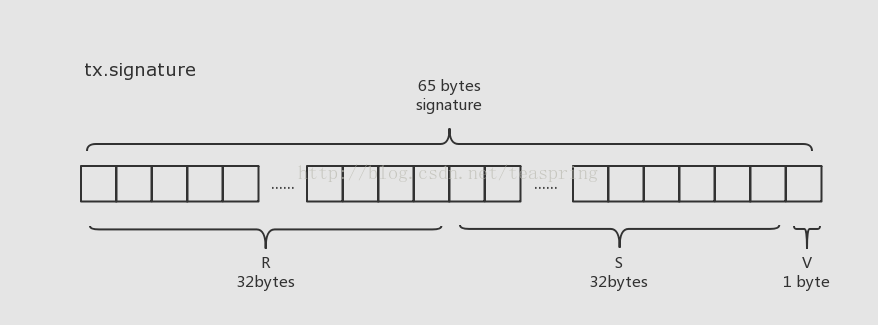
\includegraphics[scale=0.4]{signature.png}
	\caption{Signature}
	\label{signature}
\end{figure}

Ethereum 中每个交易(transaction,tx)对象在被放进block时,都是经过数字签名的,这样可以在后续传输和处理中随时验证tx是否经过篡改。Ethereum 采用的数字签名是椭圆曲线数字签名算法(Elliptic Cure Digital Signature Algorithm,ECDSA)。ECDSA 相比于基于大质数分解的RSA数字签名算法,可以在提供相同安全级别(in bits)的同时,仅需更短的公钥(public key)。关于ECDSA的算法理论和实现细节,本系列会有另外一篇文章专门加以介绍。这里需要特别留意的是,tx的转帐转出方地址,就是对该tx对象作ECDSA签名计算时所用的公钥publicKey。

Ethereum中的数字签名计算过程所生成的签名(signature), 是一个长度为65bytes的字节数组,它被截成三段放进tx中,前32bytes赋值给成员变量R, 再32bytes赋值给S,末1byte赋给V,当然由于R、S、V声明的类型都是*big.Int, 上述赋值存在[]byte -> big.Int的类型转换。

当需要恢复出tx对象的转帐转出方地址时(比如在需要执行该交易时),Ethereum 会先从tx的signature中恢复出公钥,再将公钥转化成一个common.Address类型的地址,signature由tx对象的三个成员变量R,S,V转化成字节数组[]byte后拼接得到。

Ethereum 对此定义了一个接口Signer, 用来执行挂载签名,恢复公钥,对tx对象做哈希等操作。

\begin{lstlisting}
/core/types/transaction_signing.go


// Signer encapsulates transaction signature handling. Note that this interface is not a
// stable API and may change at any time to accommodate new protocol rules.
type Signer interface {
	// Sender returns the sender address of the transaction.
	Sender(tx *Transaction) (common.Address, error)
	// SignatureValues returns the raw R, S, V values corresponding to the
	// given signature.
	SignatureValues(tx *Transaction, sig []byte) (r, s, v *big.Int, err error)
	// Hash returns the hash to be signed.
	Hash(tx *Transaction) common.Hash
	// Equal returns true if the given signer is the same as the receiver.
	Equal(Signer) bool
}
\end{lstlisting}

生成数字签名的函数叫SignTx(),它会先调用其他函数生成signature, 然后调用tx.WithSignature()将signature分段赋值给tx的成员变量R,S,V。

\begin{lstlisting}
func SignTx(tx *Transaction, s Signer, prv *ecdsa.PrivateKey) (*Transaction, error)
\end{lstlisting}

恢复出转出方地址的函数叫Sender(), 参数包括一个Signer, 一个Transaction,代码如下:

\begin{lstlisting}
func Sender(signer Signer, tx *Transaction) (common.Address, error) {  
    if sc := tx.from().Load(); sc != null {  
        sigCache := sc.(sigCache)// cache exists,  
        if sigCache.signer.Equal(signer) {  
            return sigCache.from, nil  
        }   
    }  
    addr, err := signer.Sender(tx)  
    if err != nil {  
        return common.Address{}, err  
    }  
    tx.from.Store(sigCache{signer: signer, from: addr}) // cache it  
    return addr, nil  
}  
\end{lstlisting}

Sender()函数体中,signer.Sender()会从本次数字签名的签名字符串(signature)中恢复出公钥,并转化为tx的(转帐)转出方地址。
在上文提到的ApplyTransaction()实现中,Transaction对象需要首先被转化成Message接口,用到的AsMessage()函数即调用了此处的Sender()。


\begin{lstlisting}
// core/types/transaction.go  
func (tx *Transaction) AsMessage(s Signer) (Message,error) {  
    msg := Message{  
        price: new(big.Int).Set(tx.data.price)  
        gasLimit: new(big.Int).Set(tx.data.GasLimit)  
        ...  
    }  
    var err error  
    msg.from, err = Sender(s, tx)  
    return msg, err  
}
\end{lstlisting}

在Transaction对象tx的转帐转出方地址被解析出以后,tx 就被完全转换成了Message类型,可以提供给虚拟机EVM执行了。

\subsection{交易池}


\subsection{交易执行}

参考:https://blog.csdn.net/teaspring/article/details/75389151

\Emph{虚拟机外}

执行tx的入口函数是StateProcessor的Process()函数,其代码如下:

\begin{lstlisting}
/core/state_processor.go
// Process processes the state changes according to the Ethereum rules 
// by running the transaction messages using the statedb
// and applying any rewards to both the processor (coinbase) 
// and any included uncles.
//
// Process returns the receipts and logs accumulated during the process
// and returns the amount of gas that was used in the process. 
// If any of the transactions failed to execute due to insufficient gas 
// it will return an error.
func (p *StateProcessor) Process(block *types.Block, statedb *state.StateDB, cfg vm.Config) (types.Receipts, []*types.Log, uint64, error) {
  var (
    receipts types.Receipts
    usedGas  = new(uint64)
    header   = block.Header()
    allLogs  []*types.Log
    gp       = new(GasPool).AddGas(block.GasLimit())
  )
  // Mutate the the block and state according to any hard-fork specs
  if p.config.DAOForkSupport && p.config.DAOForkBlock != nil && p.config.DAOForkBlock.Cmp(block.Number()) == 0 {
    misc.ApplyDAOHardFork(statedb)
  }
  // Iterate over and process the individual transactions
  for i, tx := range block.Transactions() {
    statedb.Prepare(tx.Hash(), block.Hash(), i)
    receipt, _, err := 
    ApplyTransaction(p.config, p.bc, nil, gp, statedb, 
	header, tx, usedGas, cfg)
    if err != nil {
      return nil, nil, 0, err
    }
    receipts = append(receipts, receipt)
    allLogs = append(allLogs, receipt.Logs...)
  }
  // Finalize the block, applying any consensus engine specific extras (e.g. block rewards)
  p.engine.Finalize(p.bc, header, statedb, block.Transactions(), block.Uncles(), receipts)

  return receipts, allLogs, *usedGas, nil
}

// ApplyTransaction attempts to apply a transaction to the given state database
// and uses the input parameters for its environment. It returns the receipt
// for the transaction, gas used and an error if the transaction failed,
// indicating the block was invalid.
func ApplyTransaction(config *params.ChainConfig, bc *BlockChain, author *common.Address, gp *GasPool, statedb *state.StateDB, header *types.Header, tx *types.Transaction, usedGas *uint64, cfg vm.Config) (*types.Receipt, uint64, error) {
	msg, err := tx.AsMessage(types.MakeSigner(config, header.Number))
	if err != nil {
		return nil, 0, err
	}
	// Create a new context to be used in the EVM environment
	context := NewEVMContext(msg, header, bc, author)
	// Create a new environment which holds all relevant information
	// about the transaction and calling mechanisms.
	vmenv := vm.NewEVM(context, statedb, config, cfg)
	// Apply the transaction to the current state (included in the env)
	_, gas, failed, err := ApplyMessage(vmenv, msg, gp)
	if err != nil {
		return nil, 0, err
	}
	// Update the state with pending changes
	var root []byte
	if config.IsByzantium(header.Number) {
		statedb.Finalise(true)
	} else {
		root = statedb.IntermediateRoot(config.IsEIP158(header.Number)).Bytes()
	}
	*usedGas += gas

	// Create a new receipt for the transaction, storing the intermediate root and gas used by the tx
	// based on the eip phase, we're passing wether the root touch-delete accounts.
	receipt := types.NewReceipt(root, failed, *usedGas)
	receipt.TxHash = tx.Hash()
	receipt.GasUsed = gas
	// if the transaction created a contract, store the creation address in the receipt.
	if msg.To() == nil {
		receipt.ContractAddress = crypto.CreateAddress(vmenv.Context.Origin, tx.Nonce())
	}
	// Set the receipt logs and create a bloom for filtering
	receipt.Logs = statedb.GetLogs(tx.Hash())
	receipt.Bloom = types.CreateBloom(types.Receipts{receipt})

	return receipt, gas, err
}
\end{lstlisting}

\begin{figure}
	\centering
	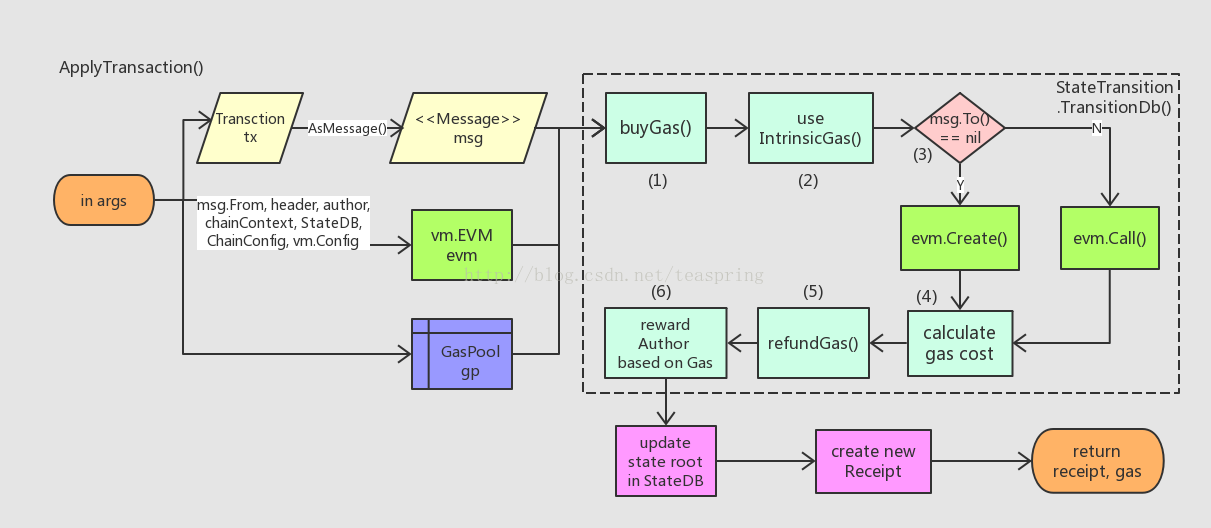
\includegraphics[scale=0.3]{applyTransaction.png}
	\caption{ApplyTransaction}
	\label{applyTransaction}
\end{figure}

\paragraph{GasPool}
GasPool类型是big.Int,在一个Block的处理过程中(即其所有tx的执行过程)中,GasPool的值能够告诉你,剩下还有多少Gas可以使用。
在每一个tx执行过程中,以太坊还设计了偿退(refund)环节,所refund的Gas数量也会加到这个GasPool里。

Process()函数的核心是一个for循环,它将Block里的所有tx遍历执行。具体的执行函数ApplyTransaction(),它每次执行tx,会返回一个收据(Receipt)对象。

ApplyTransaction()首先根据输入参数分别封装出一个Message对象和一个EVM对象,然后加上一个传入的GasPool类型变量,由TransitionDb()函数完成tx的执行,待TransitionDb()返回之后,创建一个收据Receipt对象,最后返回该Recetip对象,以及整个tx执行过程所消耗Gas数量。

GasPool对象是在一个Block执行开始时创建,并在该Block内所有tx的执行过程中共享,对于一个tx的执行可视为“全局”存储对象; Message由此次待执行的tx对象转化而来,并携带了解析出的tx的(转帐)转出方地址,属于待处理的数据对象;EVM 作为Ethereum世界里的虚拟机(Virtual Machine),作为此次tx的实际执行者,完成转帐和合约(Contract)的相关操作。

我们来细看下TransitioinDb()的执行过程(/core/state\_transition.go)。假设有StateTransition对象st,其成员变量initialGas表示初始可用Gas数量,gas表示即时可用Gas数量,初始值均为0,于是st.TransitionDb() 可由以下步骤展开:

\begin{itemize}
	\item 1. 购买Gas。首先从交易的(转帐)转出方账户扣除一笔Ether,费用等于tx.data.GasLimit * tx.data.Price;同时 st.initialGas = st.gas = tx.data.GasLimit;然后(GasPool) gp -= st.gas。

	\item 2. 计算tx的固有Gas消耗 - intrinsicGas。它分为两个部分,每一个tx预设的消耗量,这个消耗量还因tx是否含有(转帐)转入方地址而略有不同;以及针对tx.data.Payload的Gas消耗,Payload类型是[]byte,关于它的固有消耗依赖于[]byte中非0字节和0字节的长度。最终,st.gas -= intrinsicGas

	\item 3. EVM执行。如果交易的(转帐)转入方地址(tx.data.Recipient)为空,调用EVM的Create()函数;否则,调用Call()函数。无论哪个函数返回后,更新st.gas。

	\item 4. 计算本次执行交易的实际Gas消耗: requiredGas = st.initialGas - st.gas

	\item 5. 偿退Gas。它包括两个部分:首先将剩余st.gas 折算成Ether,归还给交易的(转帐)转出方账户;然后,基于实际消耗量requiredGas,系统提供一定的补偿,数量为refundGas。refundGas 所折算的Ether会被立即加在(转帐)转出方账户上,同时st.gas += refundGas,gp += st.gas,即剩余的Gas加上系统补偿的Gas,被一起归并进GasPool,供之后的交易执行使用。

	\item 6. 奖励所属区块的挖掘者:系统给所属区块的作者,亦即挖掘者账户,增加一笔金额,数额等于 st.data,Price * (st.initialGas - st.gas)。注意,这里的st.gas在步骤5中被加上了refundGas, 所以这笔奖励金所对应的Gas,其数量小于该交易实际消耗量requiredGas。
\end{itemize}
由上可见,除了步骤3中EVM 函数的执行,其他每个步骤都在围绕着Gas消耗量作文章(EVM 虚拟机的运行原理容后再述)。到这里,大家可以对Gas在以太坊系统里的作用有个初步概念,Gas就是Ethereum系统中的血液。

步骤5的偿退机制很有意思,设立它的目的何在?目前为止我只能理解它可以避免交易执行过程中过快消耗Gas,至于对其全面准确的理解尚需时日。

步骤6就更有趣了,正是这个奖励机制的存在,才会吸引社会上的矿工(miner)去卖力“挖矿”(mining)。越大的运算能力带来越多的的区块(交易)产出,矿工也就能通过该奖励机制赚取越多的以太币。

\begin{lstlisting}

/core/state_transition.go

// ApplyMessage computes the new state by applying the given message
// against the old state within the environment.
//
// ApplyMessage returns the bytes returned by any EVM execution (if it took place),
// the gas used (which includes gas refunds) and an error if it failed. An error always
// indicates a core error meaning that the message would always fail for that particular
// state and would never be accepted within a block.
func ApplyMessage(evm *vm.EVM, msg Message, gp *GasPool) ([]byte, uint64, bool, error) {
	return NewStateTransition(evm, msg, gp).TransitionDb()
}
\end{lstlisting}

\begin{lstlisting}

/core/types/receipt.go

// Receipt represents the results of a transaction.
type Receipt struct {
	// Consensus fields
	PostState         []byte `json:"root"`
	Status            uint64 `json:"status"`
	CumulativeGasUsed uint64 `json:"cumulativeGasUsed" gencodec:"required"`
	Bloom             Bloom  `json:"logsBloom"         gencodec:"required"`
	Logs              []*Log `json:"logs"              gencodec:"required"`

	// Implementation fields (don't reorder!)
	TxHash          common.Hash    `json:"transactionHash" gencodec:"required"`
	ContractAddress common.Address `json:"contractAddress"`
	GasUsed         uint64         `json:"gasUsed" gencodec:"required"`
}
\end{lstlisting}

\Emph{虚拟机内}

每个交易(Transaction)带有两部分内容需要执行:1. 转帐,由转出方地址向转入方地址转帐一笔以太币Ether; 2. 携带的[]byte类型成员变量Payload,其每一个byte都对应了一个单独虚拟机指令。这些内容都是由EVM(Ethereum Virtual Machine)对象来完成的。EVM 结构体是Ethereum虚拟机机制的核心,它与协同类的UML关系图如下:

\begin{figure}[ht]
	\centering
	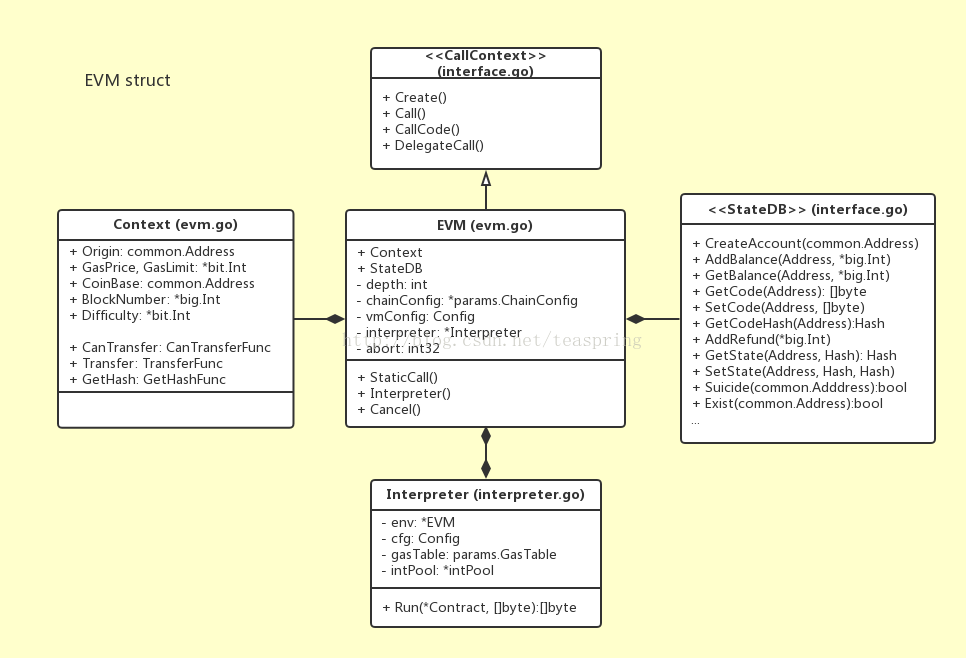
\includegraphics[scale=0.3]{evm.png}
	\caption{EVM}
	\label{evm}
\end{figure}

其中Context结构体分别携带了Transaction的信息(GasPrice, GasLimit),Block的信息(Number, Difficulty),以及转帐函数等,提供给EVM;StateDB 接口是针对state.StateDB 结构体设计的本地行为接口,可为EVM提供statedb的相关操作; Interpreter结构体作为解释器,用来解释执行EVM中合约(Contract)的指令(Code)。

注意,EVM 中定义的成员变量Context和StateDB, 仅仅声明了变量名而无类型,而变量名同时又是其类型名,在Golang中,这种方式意味着宗主结构体可以直接调用该成员变量的所有方法和成员变量,比如EVM调用Context中的Transfer()。

详情:https://blog.csdn.net/teaspring/article/details/75389151

\ifx\allfiles\undefined
\end{document}
\fi